\let\negmedspace\undefined
\let\negthickspace\undefined
\documentclass[journal]{IEEEtran}
\usepackage[a4paper, margin=10mm, onecolumn]{geometry}
%\usepackage{lmodern} % Ensure lmodern is loaded for pdflatex
\usepackage{tfrupee} % Include tfrupee package

\setlength{\headheight}{1cm} % Set the height of the header box
\setlength{\headsep}{0mm}  % Set the distance between the header box and the top of the text

\usepackage{gvv-book}
\usepackage{gvv}
\usepackage{cite}
\usepackage{amsmath,amssymb,amsfonts,amsthm}
\usepackage{algorithmic}
\usepackage{graphicx}
\usepackage{float}
\usepackage{textcomp}
\usepackage{xcolor}
\usepackage{txfonts}
\usepackage{listings}
\usepackage{enumitem}
\usepackage{mathtools}
\usepackage{gensymb}
\usepackage{comment}
\usepackage[breaklinks=true]{hyperref}
\usepackage{tkz-euclide} 
\usepackage{listings}
% \usepackage{gvv}                                        
\def\inputGnumericTable{}                                 
\usepackage[latin1]{inputenc}                                
\usepackage{color}                                            
\usepackage{array}                                            
\usepackage{longtable}                                       
\usepackage{calc}                                             
\usepackage{multirow}                                         
\usepackage{hhline}                                           
\usepackage{ifthen}                                           
\usepackage{lscape}
\usepackage{tikz}
\usetikzlibrary{patterns}

\begin{document}

\bibliographystyle{IEEEtran}
\vspace{3cm}

\title{10.7.111}
\author{ee25btech11063-vejith}

\maketitle
% \maketitle
% \newpage
% \bigskip
{\let\newpage\relax\maketitle}
\renewcommand{\thefigure}{\theenumi}
\renewcommand{\thetable}{\theenumi}
\setlength{\intextsep}{10pt} % Space between text and floats
\textbf{Question}:\\
Let the straight line $y = 2x$ touch a circle with center $(0, a)$, $a > 0$, and radius $r$ at a point $\vec{A_1}$. Let $\vec{B_1}$ be the point on the circle such that the line segment $\vec{A_1}\vec{B_1}$ is a diameter of the circle. Let $a + r = 5 + \sqrt{5}$. Match the following:\\

\begin{tabular}{ l l }

(A) $a$ equals & (1) \brak{-2,4}\\
(B)  r equals & 2. $\sqrt{5}$\\
(C)$\vec{A_1}$ equals  & (3)\brak{-2,6}\\
(D) $\vec{B_1}$ equals & (4) 5\\
	& (5) \brak{2,4}\\
\end{tabular}\\

The correct option is \hspace{15cm} \brak{2024}
\begin{enumerate}[label=\alph*)]

    \item A$- 4$, B$- 2$, C$- 1$, D$- 3$
    \item A$- 2$, B$- 4$, C$- 1$, D$- 3$
    \item A$- 4$, B$- 2$, C$- 5$, D$- 3$
    \item A$- 2$, B$- 4$, C$- 3$, D$- 5$
\end{enumerate}

\textbf{Solution}:\\
The equation of a Conic in Matrix form is
\begin{align}
\vec{x}^\top\vec{V}\vec{x} + 2\vec{u}^\top\vec{x} + f = 0
\end{align}
For the given circle. let $r$ be the radius of given circle 
\begin{align}
    \vec{V}=\begin{pmatrix}
        1 & 0\\
        0 & 1
    \end{pmatrix},\vec{u}=\myvec{0\\-a},f=a^2-r^2
\end{align}
Equation of Tangent is given by
\begin{align}
    \vec{n}^\top\vec{x}=c\\
    \implies \vec{n}=\myvec{2\\-1} ,c=0\\
    \implies \brak{2\hspace{0.5cm}-1}\myvec{x\\y}=0
\end{align}
The distance of point $\vec{P}$ to the line $\vec{n}^\top\vec{x}=c$ is given by
\begin{align}
    d=\frac{|\vec{n}^\top\vec{P}-c|}{\norm{\vec{n}}}\\
    \implies r = \frac{\left\lvert
\begin{pmatrix} 2 & 1 \end{pmatrix}
\begin{pmatrix} 0 \\ -a \end{pmatrix} - 0
\right\rvert}{\sqrt{5}}\\
\implies r=\frac{a}{\sqrt{5}}
\end{align}
\begin{align}
a + r = 5 + \sqrt{5}
\end{align}
substitute (8) in (9)
\begin{align}
\sqrt{5}r +r =5 +\sqrt{5}\\
    \implies r=\sqrt{5}\\
    \implies a=5
\end{align}
For a circle, the points of contact are
\begin{align}
    \vec{q_{j}}=\brak{\pm r \frac{\vec{n_j}}{\norm{\vec{n_j}}}-\vec{u}},j=1,2
\end{align}
let $\vec{A_1}$ be the point of contact
\begin{align}
    \vec{A_1}=\brak{-r \frac{\vec{n}}{\norm{\vec{n}}}-\vec{u}}\\
    =\brak{\frac{r}{\sqrt{5}}\myvec{2\\-1}-\myvec{0\\-a}} \hspace{0.5cm}\\ 
    \implies \vec{A_1}=\myvec{2\\4}
\end{align}

    Given  $\vec{A_1}$ and $\vec{B_1}$ is the diameter of the circle 
\begin{align}
    \frac{\vec{A_1}+\vec{B_1}}{2}=\vec{u}\\
    \vec{B_1}=\brak{\vec{u} \hspace{0.5cm} \vec{A_1}}\myvec{2\\-1}\\
    \vec{B_1}=\myvec{-2\\6}
\end{align}
Answer is c) A$- 4$, B$- 2$, C$- 5$, D$- 3$
\begin{figure}[h!]
    \centering
    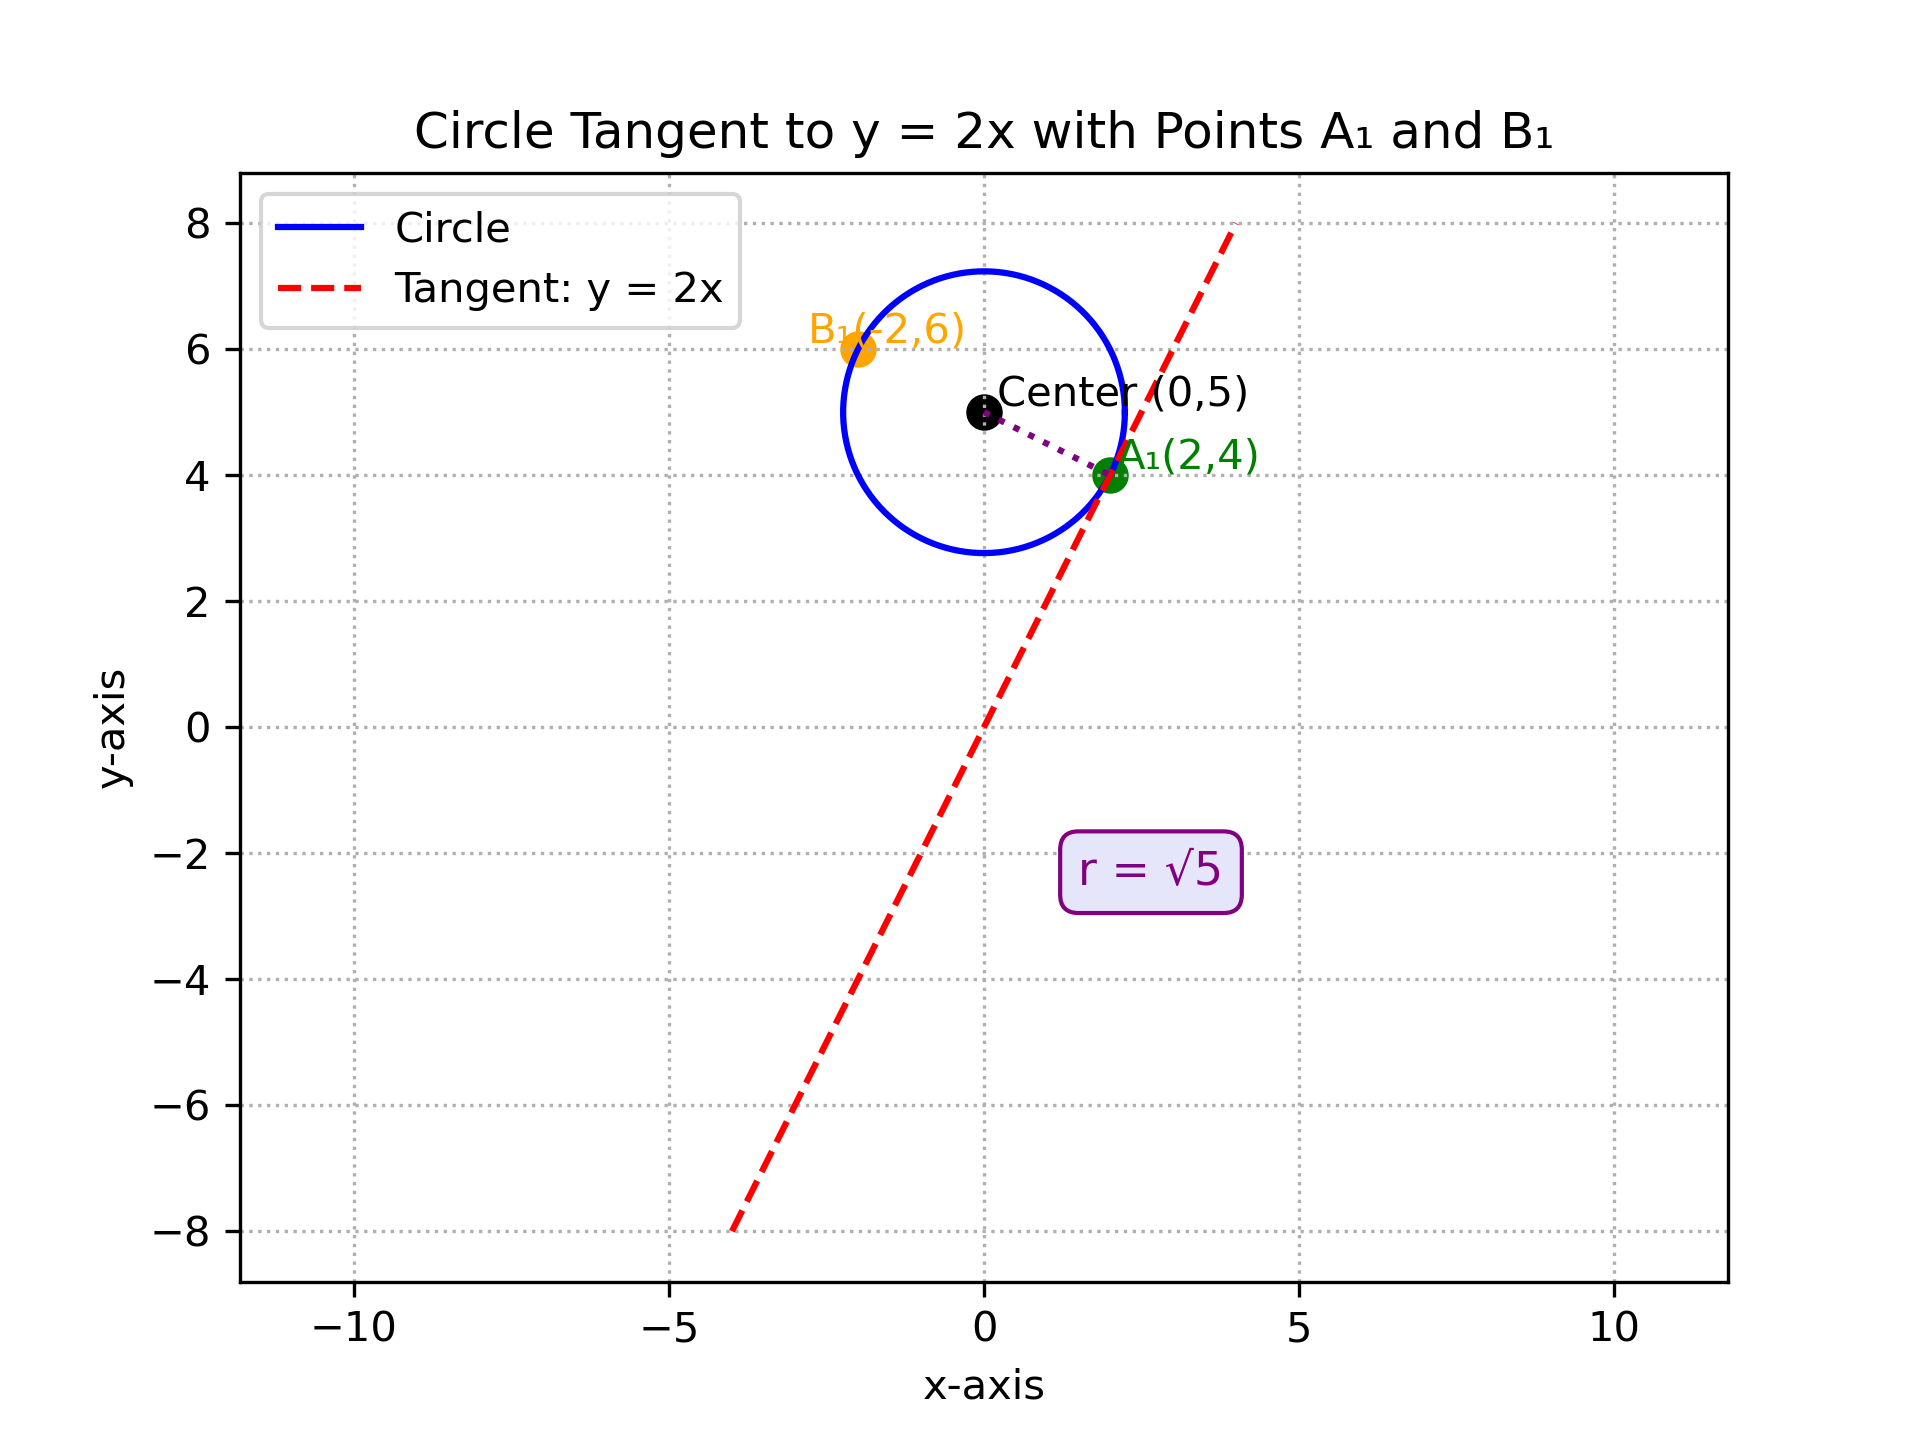
\includegraphics[width=0.8\columnwidth]{figs/01.png}
    \caption{}
    \label{fig:placeholder}
\end{figure}
\end{document}
